% 05-unsupervised-learning-clustering.tex

% Unsupervised Learning – Clustering
% 5.1. Introduction: Provides an overview of the clustering task and its objectives.
% 5.2. Determine the Number of Clusters: Uses methods like the elbow method or silhouette analysis to determine the number of clusters.
% 5.3. Hyperparameter Tuning: Tunes other hyperparameters, if any.
% 5.4. Cluster Visualization: Visualizes the clusters through t-SNE.
% 5.5. Cluster Analysis: Analyzes the characteristics of each cluster.
% 5.6. Intent Homogeneity: Assesses if clusters reflect intent division.
% 5.7. Specific Attack Categories: Associates clusters with specific attack categories.

% Section Title

\subsection*{Introduction}
This section of the project focuses on applying unsupervised learning techniques to analyze SSH attack data. Specifically, clustering methods were utilized to uncover patterns and relationships within the dataset. An emphasis was placed on identifying distinct attack behaviors and intents.

\subsection*{Data Preparation}
The dataset chosen was the one generated through the TF-IDF vectorization technique. This was made because it was essential to start with a dataset that represented in the best way the frequency and the importance of words, making each word as a dimension of our vector.

\subsection*{Clustering Methods}
Two clustering techniques were applied:
\begin{itemize}
    \item \textbf{K-Means Clustering}: Using the Elbow Method and silhouette scores, the optimal number of clusters was determined.
    \item \textbf{Gaussian Mixture Model (GMM)}: Similar to K-Means, the optimal number of clusters was selected using silhouette scores and log-likelihood values.
\end{itemize}

\subsection*{Hyperparameter Tuning}
Hyperparameter tuning was conducted to optimize the performance of both clustering methods. For K-Means, parameters such as the initialization method (\texttt{k-means++} and \texttt{random}), the number of initializations, and the maximum number of iterations were fine-tuned using a grid search approach. Similarly, GMM parameters including the initialization method (\texttt{kmeans}), covariance type (\texttt{full} and \texttt{spherical}), and tolerance were optimized. These steps ensured the models were tailored to the dataset, resulting in better clustering outcomes.

\subsection*{Clusters Visualization}
To visualize the clustering results, t-SNE dimensionality reduction was applied. Its functionalities makes it an excellent choice for visualizing clusters in datasets where direct interpretation is difficult due to high dimensionality. By projecting the data into a two-dimensional space, t-SNE enables us to identify patterns and groupings that may not be evident in the original feature space. The two-dimensional plots provided a clear representation of the clusters formed by both K-Means and GMM, highlighting their separability and internal consistency.


\subsubsection*{K-Means Visualization}
\begin{figure}[H]
    \centering
    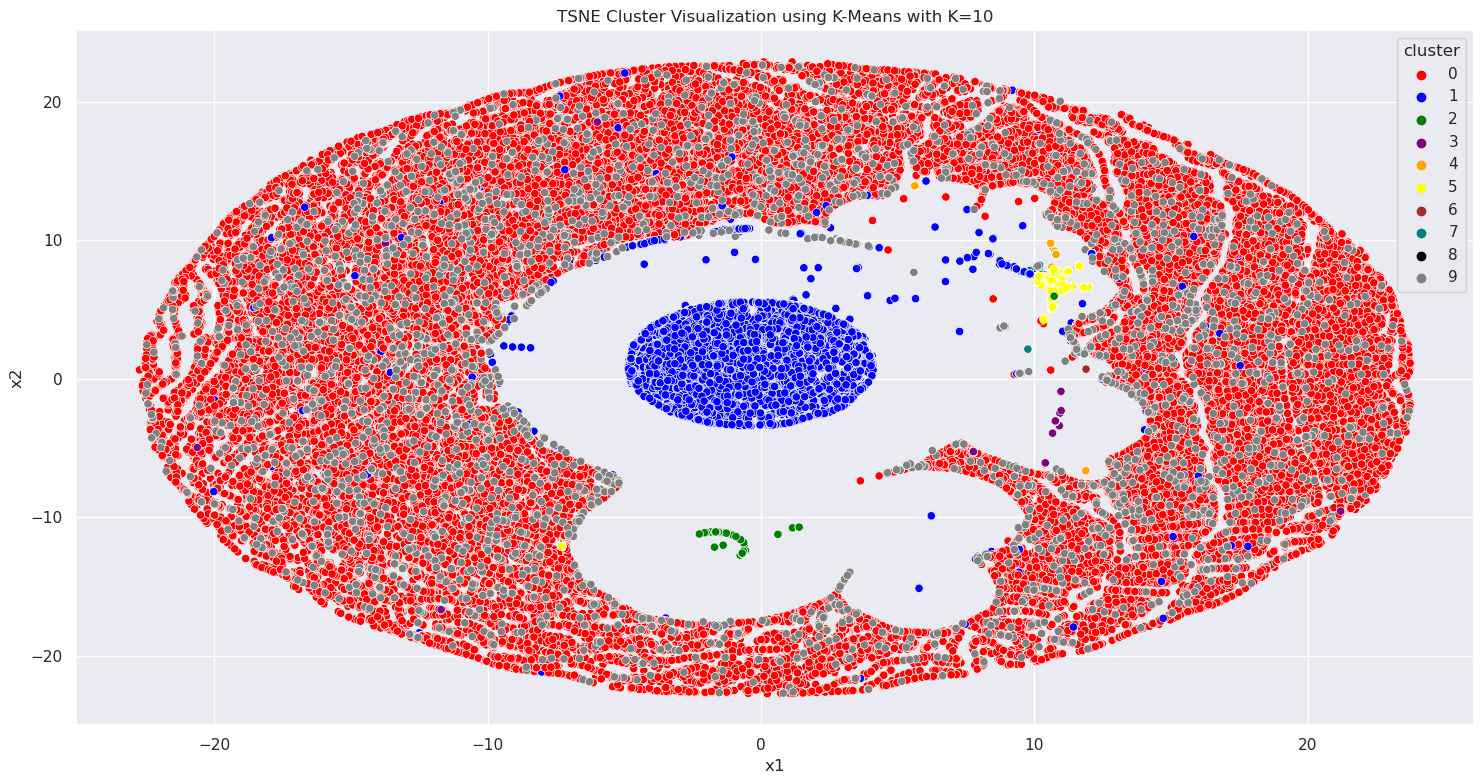
\includegraphics[width=0.8\textwidth]{../figures/plots/section3/tsne_kmeans_clusters.png}
    \caption{t-SNE Visualization of K-Means Clusters.}
    \label{fig:tsne_kmeans}
\end{figure}

\subsubsection*{GMM Visualization}
\begin{figure}[H]
    \centering
    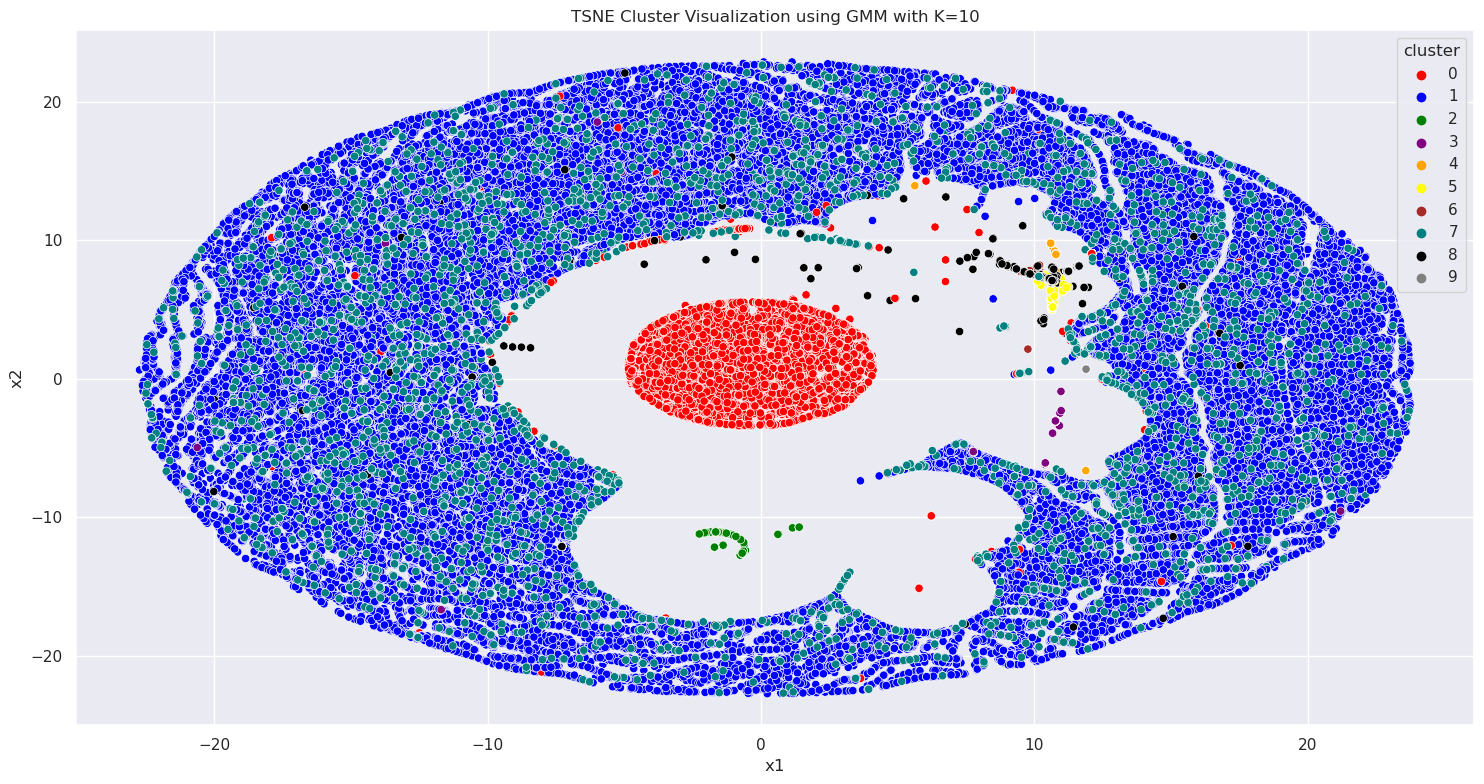
\includegraphics[width=0.8\textwidth]{../figures/plots/section3/tsne_gmm_clusters.png}
    \caption{t-SNE Visualization of GMM Clusters.}
    \label{fig:tsne_gmm}
\end{figure}

\subsection*{Clusters Analysis}

\subsubsection*{Word Cloud Representation}
Word clouds were generated for each cluster to highlight the most significant terms. This provided an intuitive understanding of the key features within each cluster, offering insights into the behavioral patterns of the attacks.

\begin{figure}[H]
    \centering
    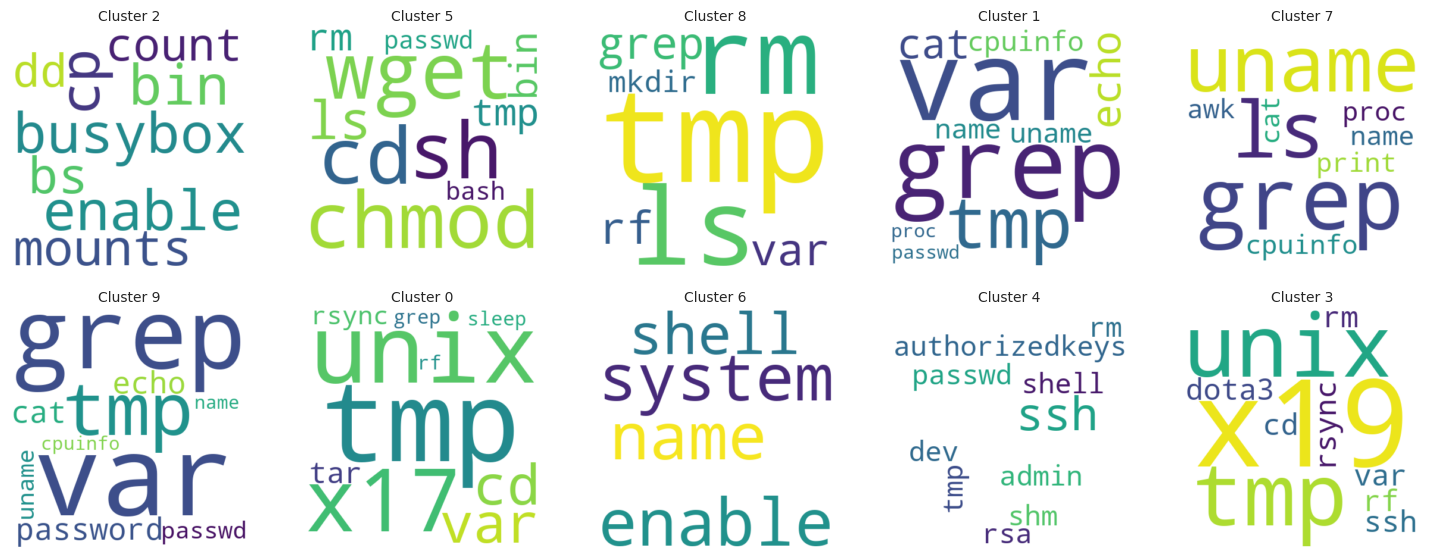
\includegraphics[width=0.9\textwidth]{../figures/plots/section3/circular_wordclouds.png}
    \caption{Word Clouds for Each Cluster.}
    \label{fig:word_clouds}
\end{figure}

\subsubsection*{Community Detection}
Graph-based community detection was performed within selected clusters to identify subgroups. The analysis revealed meaningful relationships and substructures within the data, as demonstrated in the visualizations below:

\begin{figure}[H]
    \centering
    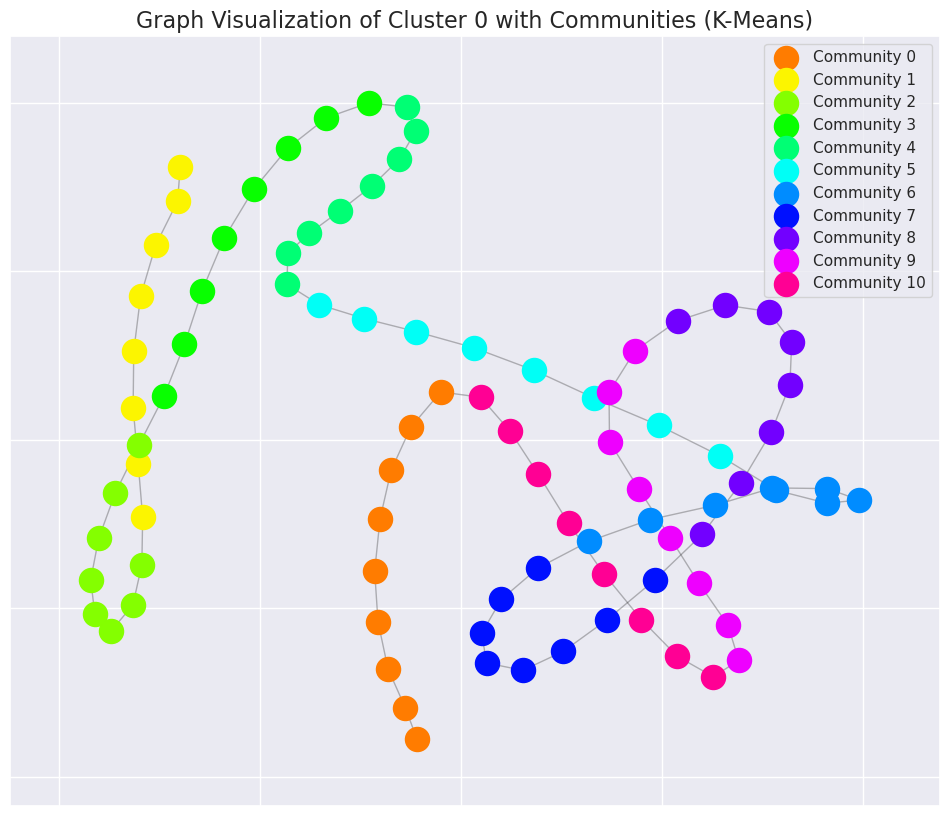
\includegraphics[width=0.8\textwidth]{../figures/plots/section3/k-means_graph_visualization_of_cluster_0_with_communities.png}
    \caption{Community Detection in Cluster 0 (K-Means).}
    \label{fig:kmeans_graph}
\end{figure}

\begin{figure}[H]
    \centering
    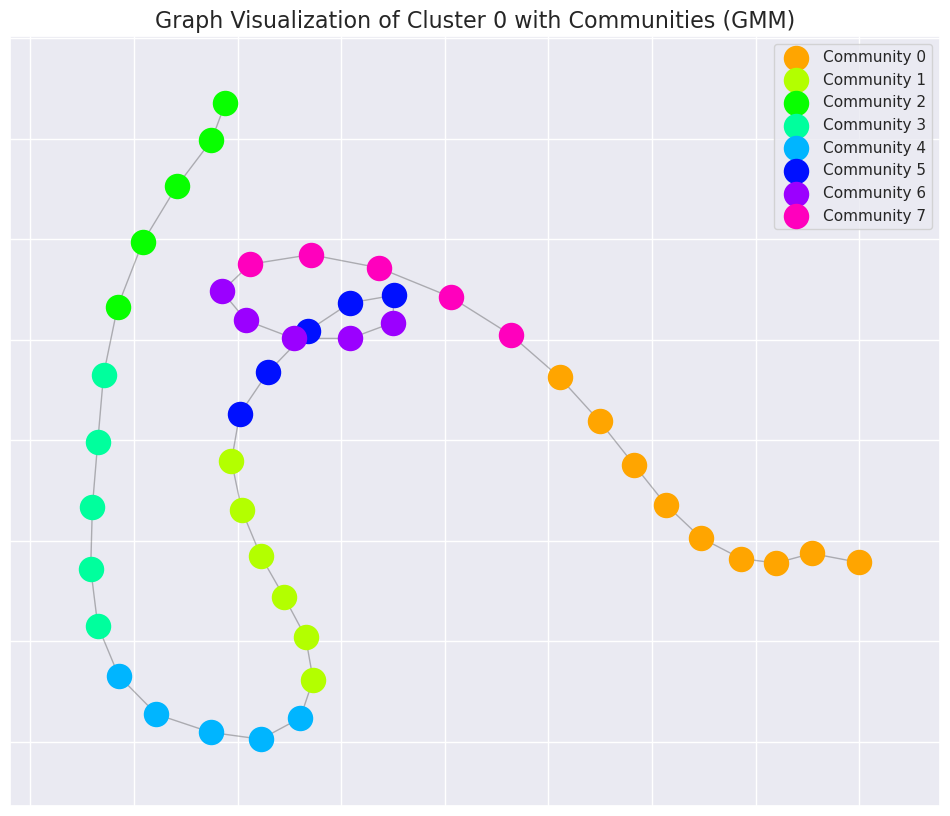
\includegraphics[width=0.8\textwidth]{../figures/plots/section3/gmm_graph_visualization_of_cluster_0_with_communities.png}
    \caption{Community Detection in Cluster 0 (GMM).}
    \label{fig:gmm_graph}
\end{figure}

\subsection*{Conclusion}
This analysis provided valuable insights into the patterns of SSH attacks through clustering. The K-Means and GMM algorithms both effectively identified meaningful clusters, as supported by validation metrics and visualizations. Hyperparameter tuning further enhanced the performance of both models. The results demonstrate the potential of unsupervised learning in uncovering hidden patterns in complex datasets, providing a foundation for future applications such as anomaly detection and improved cybersecurity strategies.

